\begin{withoutheadline}
  \begin{frame}{From physics to the mathematical model}
  \vspace{-0.6cm}
  \begin{overprint}
    \onslide<1>
    
    \begin{columns}
      \begin{column}{0.45\textwidth}
        \begin{block}{Solid dynamics problems}
          \begin{itemize}
          \item[] Impact; Crash-proof design
          \item[] \textbf{High-speed forming}
          \end{itemize}
        \end{block}
      \end{column}
      
      \begin{column}{0.55\textwidth}
      \end{column}
    \end{columns}

    
    \begin{columns}
      \begin{column}{0.45\textwidth}
        \centering
        \movie[height = 0.3275\paperheight,width=0.6\linewidth,loop,poster,autostart]{}{%
      section1/animation/output3.mp4}\\
    \scriptsize Electromagnetic forming \cite{Guillaume}
      \end{column}
      \begin{column}{0.45\textwidth}
        \begin{block}{}
          \begin{footnotesize}
            \begin{itemize}
            \item Complex geometries
            \item Irreversible strains
            \item High-velocity ($\approx \: 50\:\text{m/s}$) $\rightarrow$ waves
            \item[]
            \item[]
            \item[]
            \end{itemize}
          \end{footnotesize}
        \end{block}  
      \end{column}
    \end{columns}
    \footnoteCite{Guillaume}
    
    \onslide<2>
    \begin{columns}
      \begin{column}{0.45\textwidth}
        \begin{block}{Solid dynamics problems}
          \begin{itemize}
          \item[] Impact; Crash-proof design
          \item[] High-speed forming
          \end{itemize}
        \end{block}
      \end{column}
      
      
      \begin{column}{0.55\textwidth}
        \begin{block}{Mathematical model}
          \begin{itemize}
          \item[] Partial differential equations
          \item[] Hyperbolic system
          \end{itemize}
        \end{block}
      \end{column}
    \end{columns}

    \vspace{1.cm}
    \begin{block}{Challenging task}
      \alert{Accurately track waves propagating/interacting in finite deforming elastic-plastic solids }
    \end{block}
    %% Il faut dire que suivre ces ondes est très important pour comprendre la physique et évaluer correctement les états résiduels

    \vspace{0.5cm}
    \begin{block}{Complex equations }
      \begin{columns}
        \begin{column}{0.5\textwidth}
          \begin{itemize}
          \item Large deformations
          \item Complex geometries
          \item Waves
          \end{itemize}
        \end{column}
        \begin{column}{0.5\textwidth}
          \begin{itemize}
          \item[] 
          \item[$\Rightarrow$]  Resort to numerical simulation
          \item[]
          \end{itemize}
        \end{column}
      \end{columns}
    \end{block}
    % \footnoteCite{Wang}
  \end{overprint}
\end{frame}\end{withoutheadline}


\begin{withoutheadline}
  \begin{frame}{Some explicit numerical methods}
    \vspace{-0.5cm}
    \begin{overprint}
      \onslide<1>
      \vspace{-0.65cm}
      \begin{columns}
        \begin{column}{0.49\textwidth}
          \begin{block}{The Finite Element Method \cite{Belytschko}}
            \begin{footnotesize}
              \begin{block}{\footnotesize Pros}
                \vspace{-0.2cm}
                \begin{itemize}
                \item[] Non-linear constitutive equations
                \item[] High-order approximation
                \end{itemize}
              \end{block}
              \vspace{-0.2cm}
              \begin{block}{\footnotesize Cons}
                \vspace{-0.2cm}
                \begin{itemize}
                \item[] \textbf{Oscillations near discontinuities} 
                % \item[] Lagrangian: mesh entanglement
                % \item[] Eulerian: diffusion
                \end{itemize}
              \end{block}
            \end{footnotesize}
          \end{block}
        \end{column}
        \begin{column}{0.49\textwidth}
          \begin{block}{}
            \centering
            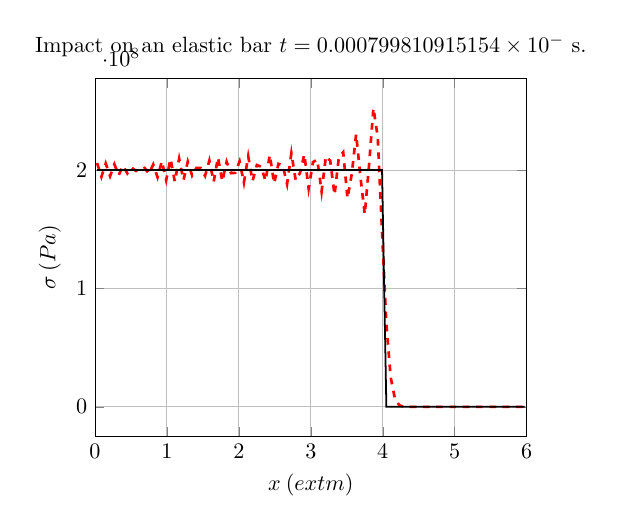
\begin{tikzpicture}[scale=0.8]
\begin{axis}[xlabel=$x \:(	ext{m})$,ylabel=$\sigma \: (\text{Pa})$,ymajorgrids=true,xmajorgrids=true,legend pos=north east,title={Impact on an elastic bar $t = 0.000799810915154\times 10^{-} $ s.},xmin=0.,xmax=6.]
\addplot[Red,very thick,mark=none,dashed] coordinates {(0.03,205801663.056) (0.09,194290281.751) (0.15,205522777.697) (0.21,194765045.219) (0.27,204837977.189) (0.33,195678091.442) (0.39,203676191.803) (0.45,197108930.16) (0.51,201959433.742) (0.57,199120873.566) (0.63,199655686.067) (0.69,201694558.408) (0.75,196858768.899) (0.81,204636822.218) (0.87,193885732.355) (0.93,207485875.371) (0.99,191355550.934) (1.05,209467570.081) (1.11,190174014.86) (1.17,209596824.204) (1.23,191318150.416) (1.29,207030033.346) (1.35,195337558.33) (1.41,201695732.551) (1.47,201641240.416) (1.53,194995238.094) (1.59,207955179.195) (1.65,189996089.745) (1.71,210691220.744) (1.77,190309615.134) (1.83,206923634.091) (1.89,197336628.108) (1.95,197581719.26) (2.01,207292315.833) (2.07,189260409.493) (2.13,211645523.176) (2.19,190620227.071) (2.25,204159086.571) (2.31,202759432.237) (2.37,190781202.887) (2.43,212737259.382) (2.49,188539123.622) (2.55,205205038.908) (2.61,203920794.53) (2.67,188137350.176) (2.73,214227015.38) (2.79,191237758.321) (2.85,197494692.379) (2.91,213192542.634) (2.97,184316952.507) (3.03,206613598.82) (3.09,208789045.003) (3.15,181765168.625) (3.21,211580666.909) (3.27,207740068.787) (3.33,178912332.687) (3.39,211007360.485) (3.45,215043311.113) (3.51,176025142.03) (3.57,196982494.169) (3.63,230309195.474) (3.69,194026599.565) (3.75,162620019.573) (3.81,204636500.028) (3.87,252350248.388) (3.93,227862374.619) (3.99,147549341.154) (4.05,70149900.687) (4.11,24899585.1034) (4.17,6624083.17904) (4.23,1307844.57053) (4.29,186564.480988) (4.35,18224.962181) (4.41,1093.2540344) (4.47,30.4203286797) (4.53,0.0) (4.59,0.0) (4.65,0.0) (4.71,0.0) (4.77,0.0) (4.83,0.0) (4.89,0.0) (4.95,0.0) (5.01,0.0) (5.07,0.0) (5.13,0.0) (5.19,0.0) (5.25,0.0) (5.31,0.0) (5.37,0.0) (5.43,0.0) (5.49,0.0) (5.55,0.0) (5.61,0.0) (5.67,0.0) (5.73,0.0) (5.79,0.0) (5.85,0.0) (5.91,0.0) (5.97,0.0) };
\addplot[black,thick,mark=none,solid] coordinates {(0.03,200000000.0) (0.09,200000000.0) (0.15,200000000.0) (0.21,200000000.0) (0.27,200000000.0) (0.33,200000000.0) (0.39,200000000.0) (0.45,200000000.0) (0.51,200000000.0) (0.57,200000000.0) (0.63,200000000.0) (0.69,200000000.0) (0.75,200000000.0) (0.81,200000000.0) (0.87,200000000.0) (0.93,200000000.0) (0.99,200000000.0) (1.05,200000000.0) (1.11,200000000.0) (1.17,200000000.0) (1.23,200000000.0) (1.29,200000000.0) (1.35,200000000.0) (1.41,200000000.0) (1.47,200000000.0) (1.53,200000000.0) (1.59,200000000.0) (1.65,200000000.0) (1.71,200000000.0) (1.77,200000000.0) (1.83,200000000.0) (1.89,200000000.0) (1.95,200000000.0) (2.01,200000000.0) (2.07,200000000.0) (2.13,200000000.0) (2.19,200000000.0) (2.25,200000000.0) (2.31,200000000.0) (2.37,200000000.0) (2.43,200000000.0) (2.49,200000000.0) (2.55,200000000.0) (2.61,200000000.0) (2.67,200000000.0) (2.73,200000000.0) (2.79,200000000.0) (2.85,200000000.0) (2.91,200000000.0) (2.97,200000000.0) (3.03,200000000.0) (3.09,200000000.0) (3.15,200000000.0) (3.21,200000000.0) (3.27,200000000.0) (3.33,200000000.0) (3.39,200000000.0) (3.45,200000000.0) (3.51,200000000.0) (3.57,200000000.0) (3.63,200000000.0) (3.69,200000000.0) (3.75,200000000.0) (3.81,200000000.0) (3.87,200000000.0) (3.93,200000000.0) (3.99,200000000.0) (4.05,0.0) (4.11,0.0) (4.17,0.0) (4.23,0.0) (4.29,0.0) (4.35,0.0) (4.41,0.0) (4.47,0.0) (4.53,0.0) (4.59,0.0) (4.65,0.0) (4.71,0.0) (4.77,0.0) (4.83,0.0) (4.89,0.0) (4.95,0.0) (5.01,0.0) (5.07,0.0) (5.13,0.0) (5.19,0.0) (5.25,0.0) (5.31,0.0) (5.37,0.0) (5.43,0.0) (5.49,0.0) (5.55,0.0) (5.61,0.0) (5.67,0.0) (5.73,0.0) (5.79,0.0) (5.85,0.0) (5.91,0.0) (5.97,0.0) };
%\legend{fem,exact}
\end{axis}
\end{tikzpicture}
%%% Local Variables:
%%% mode: latex
%%% TeX-master: "../../mainManuscript"
%%% End:

          \end{block}
        \end{column}
      \end{columns}
      \vspace{-0.25cm}
      \footnoteCite{Belytschko}
      \onslide<2>
      %\vspace{-0.58cm}
      \begin{columns}
        \begin{column}{0.49\textwidth}
          \vspace{-0.1cm}
          \begin{block}{The Finite Element Method \cite{Belytschko}}
            \begin{footnotesize}
              \begin{block}{\footnotesize Pros}
                \vspace{-0.2cm}
                \begin{itemize}
                \item[] Non-linear constitutive equations
                \item[] High-order approximation 
                \end{itemize}
              \end{block}
              \vspace{-0.2cm}
              \begin{block}{\footnotesize Cons}
                \vspace{-0.2cm}
                \begin{itemize}
                \item[] Oscillations near discontinuities
                % \item[] Lagrangian: mesh entanglement 
                % \item[] Eulerian: diffusion
                \end{itemize}
              \end{block}
            \end{footnotesize}
          \end{block}
          % \begin{block}{}
          %   \centering
          % % \begin{tikzpicture}[scale=0.4]
% \begin{groupplot}[group style={group size=1 by 1,
% ylabels at=edge left, yticklabels at=edge left,horizontal sep=2.ex,
% vertical sep=4ex,xticklabels at=edge bottom,xlabels at=edge bottom},
% ymajorgrids=true,xmajorgrids=true,enlargelimits=0,xmin=0.,xmax=6.,xlabel=$x (m)$,
% axis on top,scale only axis
% ]
% % \nextgroupplot[ylabel=$\sigma (Pa)$,title={$t = 4.17\times 10^{-4} $ s.},ymin=-1.35e9,ymax=56579516.10614197,]
% % \addplot[Blue,solid,mark=x,very thick,mark size=3pt,mark repeat=3] coordinates{(0.0,-3.2561158711216654e-07) (0.12244897959183673,-6.54162606232603e-22) (0.24489795918367346,0.0) (0.36734693877551017,3.2561158711216643e-07) (0.4897959183673469,-4.884173806682499e-07) (0.6122448979591837,-706703995.0062007) (0.7346938775510203,-739923853.3127105) (0.8571428571428571,-818114621.3278772) (0.9795918367346939,-934350667.0858994) (1.1020408163265305,-1056745717.4113452) (1.2244897959183674,-1153785079.176232) (1.346938775510204,-1213891661.9862223) (1.4693877551020407,-1243675875.166416) (1.5918367346938775,-1255667377.4619899) (1.7142857142857142,-1259628756.7765899) (1.836734693877551,-1260708382.472525) (1.9591836734693877,-1260951555.06527) (2.0816326530612246,-1260996741.6987677) (2.204081632653061,-1261003631.246593) (2.326530612244898,-1261004484.7294881) (2.4489795918367347,-1261004569.3136225) (2.571428571428571,-1261004575.8625927) (2.693877551020408,-1261004576.2443771) (2.816326530612245,-1261004576.2601426) (2.9387755102040813,-1261004576.2605536) (3.061224489795918,-1261004576.2605536) (3.183673469387755,-1261004576.2601426) (3.306122448979592,-1261004576.2443776) (3.4285714285714284,-1261004575.862593) (3.5510204081632653,-1261004569.3136227) (3.673469387755102,-1261004484.7294881) (3.7959183673469385,-1261003631.2465928) (3.9183673469387754,-1260996741.6987677) (4.040816326530612,-1260951555.0652697) (4.163265306122449,-1260708382.4725246) (4.285714285714286,-1259628756.7765894) (4.408163265306122,-1255667377.4619899) (4.530612244897959,-1243675875.1664157) (4.653061224489796,-1213891661.9862223) (4.775510204081632,-1153785079.176232) (4.8979591836734695,-1056745717.4113454) (5.020408163265306,-934350667.0858992) (5.142857142857142,-818114621.327877) (5.26530612244898,-739923853.3127109) (5.387755102040816,-706703995.0062011) (5.5102040816326525,-4.884173806682498e-07) (5.63265306122449,0.0) (5.755102040816326,-4.884173806682498e-07) (5.877551020408163,0.0) (6.0,-4.884173806682498e-07) };
% % \addplot[Purple,solid,mark=+,thick,mark size=3pt,mark repeat=3] coordinates{(0.0,-3.2561158711216654e-07) (0.12244897959183673,-6.54162606232603e-22) (0.24489795918367346,0.0) (0.36734693877551017,3.2561158711216643e-07) (0.4897959183673469,-4.884173806682499e-07) (0.6122448979591837,-710637837.2357953) (0.7346938775510203,-747893724.781927) (0.8571428571428571,-827829409.8631966) (0.9795918367346939,-936780409.853217) (1.1020408163265305,-1054073198.2499647) (1.2244897959183674,-1144128439.1849532) (1.346938775510204,-1207925723.6670742) (1.4693877551020407,-1232372577.7948787) (1.5918367346938775,-1254253728.274747) (1.7142857142857142,-1243570946.3490026) (1.836734693877551,-1268139963.2569304) (1.9591836734693877,-1248035262.8872383) (2.0816326530612246,-1268992337.693115) (2.204081632653061,-1251285653.8729925) (2.326530612244898,-1266352346.5241969) (2.4489795918367347,-1253527311.8706975) (2.571428571428571,-1264419055.233534) (2.693877551020408,-1255474245.0991223) (2.816326530612245,-1261578869.0693417) (2.9387755102040813,-1258168698.6750736) (3.061224489795918,-1258168698.6750731) (3.183673469387755,-1261578869.069342) (3.306122448979592,-1255474245.0991209) (3.4285714285714284,-1264419055.233534) (3.5510204081632653,-1253527311.870696) (3.673469387755102,-1266352346.5241973) (3.7959183673469385,-1251285653.8729923) (3.9183673469387754,-1268992337.6931143) (4.040816326530612,-1248035262.8872375) (4.163265306122449,-1268139963.2569308) (4.285714285714286,-1243570946.3490026) (4.408163265306122,-1254253728.2747467) (4.530612244897959,-1232372577.7948787) (4.653061224489796,-1207925723.6670735) (4.775510204081632,-1144128439.1849532) (4.8979591836734695,-1054073198.2499645) (5.020408163265306,-936780409.853217) (5.142857142857142,-827829409.8631967) (5.26530612244898,-747893724.7819276) (5.387755102040816,-710637837.2357956) (5.5102040816326525,-4.884173806682498e-07) (5.63265306122449,0.0) (5.755102040816326,-4.884173806682498e-07) (5.877551020408163,0.0) (6.0,-4.884173806682498e-07) };
% % \addplot[black,solid,mark=none,thin,mark size=3pt,mark repeat=3] coordinates{(0.0,-0.0) (0.12244897959183673,-0.0) (0.24489795918367346,-0.0) (0.36734693877551017,-0.0) (0.4897959183673469,-0.0) (0.6122448979591837,-700000000.0) (0.7346938775510203,-700000000.0) (0.8571428571428571,-700000000.0) (0.9795918367346939,-700000000.0) (1.1020408163265305,-1261004576.260559) (1.2244897959183674,-1261004576.260559) (1.346938775510204,-1261004576.260559) (1.4693877551020407,-1261004576.260559) (1.5918367346938775,-1261004576.260559) (1.7142857142857142,-1261004576.260559) (1.836734693877551,-1261004576.260559) (1.9591836734693877,-1261004576.260559) (2.0816326530612246,-1261004576.260559) (2.204081632653061,-1261004576.260559) (2.326530612244898,-1261004576.260559) (2.4489795918367347,-1261004576.260559) (2.571428571428571,-1261004576.260559) (2.693877551020408,-1261004576.260559) (2.816326530612245,-1261004576.260559) (2.9387755102040813,-1261004576.260559) (3.061224489795918,-1261004576.260559) (3.183673469387755,-1261004576.260559) (3.306122448979592,-1261004576.260559) (3.4285714285714284,-1261004576.260559) (3.5510204081632653,-1261004576.260559) (3.673469387755102,-1261004576.260559) (3.7959183673469385,-1261004576.260559) (3.9183673469387754,-1261004576.260559) (4.040816326530612,-1261004576.260559) (4.163265306122449,-1261004576.260559) (4.285714285714286,-1261004576.260559) (4.408163265306122,-1261004576.260559) (4.530612244897959,-1261004576.260559) (4.653061224489796,-1261004576.260559) (4.775510204081632,-1261004576.260559) (4.8979591836734695,-1261004576.260559) (5.020408163265306,-700000000.0) (5.142857142857142,-700000000.0) (5.26530612244898,-700000000.0) (5.387755102040816,-700000000.0) (5.5102040816326525,-0.0) (5.63265306122449,-0.0) (5.755102040816326,-0.0) (5.877551020408163,-0.0) (6.0,-0.0) };
% \nextgroupplot[ylabel=$\eps^p $,ymin=-0.0021,ymax=0.0,title={Elastic-plastic plane waves}]
% \addplot[Blue,solid,mark=x,very thick,mark size=3pt,mark repeat=3] coordinates{(0.0,0.0) (0.12244897959183673,0.0) (0.24489795918367346,0.0) (0.36734693877551017,0.0) (0.4897959183673469,0.0) (0.6122448979591837,-2.4267855226065594e-05) (0.7346938775510203,-0.00014452073597361284) (0.8571428571428571,-0.0004275642401009131) (0.9795918367346939,-0.0008483282066457896) (1.1020408163265305,-0.0012913872123487611) (1.2244897959183674,-0.001642660920094959) (1.346938775510204,-0.0018602413103573651) (1.4693877551020407,-0.0019680574666657586) (1.5918367346938775,-0.00201146561977191) (1.7142857142857142,-0.002025805454394895) (1.836734693877551,-0.0020297136017104972) (1.9591836734693877,-0.002030593864489664) (2.0816326530612246,-0.002030757436013639) (2.204081632653061,-0.0020307823755532774) (2.326530612244898,-0.002030785465084119) (2.4489795918367347,-0.0020307857712710334) (2.571428571428571,-0.00203078579497771) (2.693877551020408,-0.0020307857963597366) (2.816326530612245,-0.002030785796416807) (2.9387755102040813,-0.002030785796418294) (3.061224489795918,-0.002030785796418294) (3.183673469387755,-0.0020307857964168056) (3.306122448979592,-0.002030785796359739) (3.4285714285714284,-0.0020307857949777124) (3.5510204081632653,-0.002030785771271032) (3.673469387755102,-0.002030785465084119) (3.7959183673469385,-0.002030782375553277) (3.9183673469387754,-0.0020307574360136386) (4.040816326530612,-0.002030593864489664) (4.163265306122449,-0.0020297136017104964) (4.285714285714286,-0.0020258054543948927) (4.408163265306122,-0.002011465619771909) (4.530612244897959,-0.0019680574666657573) (4.653061224489796,-0.0018602413103573651) (4.775510204081632,-0.0016426609200949592) (4.8979591836734695,-0.001291387212348762) (5.020408163265306,-0.0008483282066457893) (5.142857142857142,-0.00042756424010091193) (5.26530612244898,-0.00014452073597361384) (5.387755102040816,-2.4267855226067292e-05) (5.5102040816326525,0.0) (5.63265306122449,0.0) (5.755102040816326,0.0) (5.877551020408163,0.0) (6.0,0.0) };
% \addplot[Purple,solid,mark=+,thick,mark size=3pt,mark repeat=3] coordinates{(0.0,0.0) (0.12244897959183673,0.0) (0.24489795918367346,0.0) (0.36734693877551017,0.0) (0.4897959183673469,0.0) (0.6122448979591837,-3.850800809337606e-05) (0.7346938775510203,-0.00017337094943683953) (0.8571428571428571,-0.00046273089543238553) (0.9795918367346939,-0.000857123655577256) (1.1020408163265305,-0.0012817129348415013) (1.2244897959183674,-0.0016077047572306) (1.346938775510204,-0.0018386451535459692) (1.4693877551020407,-0.0019271405531036338) (1.5918367346938775,-0.002006348337646142) (1.7142857142857142,-0.002018045326373221) (1.836734693877551,-0.002056615251608797) (1.9591836734693877,-0.0020613216365693464) (2.0816326530612246,-0.002064203896841495) (2.204081632653061,-0.0020644266901542695) (2.326530612244898,-0.0020621094945296272) (2.4489795918367347,-0.002062767607181189) (2.571428571428571,-0.002061489252343496) (2.693877551020408,-0.0020573197208032658) (2.816326530612245,-0.0020502799029179) (2.9387755102040813,-0.0020377776694292327) (3.061224489795918,-0.0020377776694292327) (3.183673469387755,-0.002050279902917899) (3.306122448979592,-0.002057319720803265) (3.4285714285714284,-0.0020614892523434956) (3.5510204081632653,-0.0020627676071811878) (3.673469387755102,-0.0020621094945296285) (3.7959183673469385,-0.0020644266901542695) (3.9183673469387754,-0.0020642038968414953) (4.040816326530612,-0.0020613216365693477) (4.163265306122449,-0.002056615251608799) (4.285714285714286,-0.0020180453263732205) (4.408163265306122,-0.0020063483376461405) (4.530612244897959,-0.0019271405531036334) (4.653061224489796,-0.0018386451535459673) (4.775510204081632,-0.0016077047572305996) (4.8979591836734695,-0.0012817129348415002) (5.020408163265306,-0.0008571236555772557) (5.142857142857142,-0.000462730895432386) (5.26530612244898,-0.0001733709494368422) (5.387755102040816,-3.850800809337776e-05) (5.5102040816326525,0.0) (5.63265306122449,0.0) (5.755102040816326,0.0) (5.877551020408163,0.0) (6.0,0.0) };
% \addplot[black,solid,mark=none,thin,mark size=3pt,mark repeat=3] coordinates{(0.0,-0.0) (0.12244897959183673,-0.0) (0.24489795918367346,-0.0) (0.36734693877551017,-0.0) (0.4897959183673469,-0.0) (0.6122448979591837,-0.0) (0.7346938775510203,-0.0) (0.8571428571428571,-0.0) (0.9795918367346939,-0.0) (1.1020408163265305,-0.002030785796418313) (1.2244897959183674,-0.002030785796418313) (1.346938775510204,-0.002030785796418313) (1.4693877551020407,-0.002030785796418313) (1.5918367346938775,-0.002030785796418313) (1.7142857142857142,-0.002030785796418313) (1.836734693877551,-0.002030785796418313) (1.9591836734693877,-0.002030785796418313) (2.0816326530612246,-0.002030785796418313) (2.204081632653061,-0.002030785796418313) (2.326530612244898,-0.002030785796418313) (2.4489795918367347,-0.002030785796418313) (2.571428571428571,-0.002030785796418313) (2.693877551020408,-0.002030785796418313) (2.816326530612245,-0.002030785796418313) (2.9387755102040813,-0.002030785796418313) (3.061224489795918,-0.002030785796418313) (3.183673469387755,-0.002030785796418313) (3.306122448979592,-0.002030785796418313) (3.4285714285714284,-0.002030785796418313) (3.5510204081632653,-0.002030785796418313) (3.673469387755102,-0.002030785796418313) (3.7959183673469385,-0.002030785796418313) (3.9183673469387754,-0.002030785796418313) (4.040816326530612,-0.002030785796418313) (4.163265306122449,-0.002030785796418313) (4.285714285714286,-0.002030785796418313) (4.408163265306122,-0.002030785796418313) (4.530612244897959,-0.002030785796418313) (4.653061224489796,-0.002030785796418313) (4.775510204081632,-0.002030785796418313) (4.8979591836734695,-0.002030785796418313) (5.020408163265306,-0.0) (5.142857142857142,-0.0) (5.26530612244898,-0.0) (5.387755102040816,-0.0) (5.5102040816326525,-0.0) (5.63265306122449,-0.0) (5.755102040816326,-0.0) (5.877551020408163,-0.0) (6.0,-0.0) };

% \addlegendentry{fvm (elastic-plastic Riemann solver)}
% \addlegendentry{fvm (elastic Riemann solver)}
% \addlegendentry{exact}

% \end{groupplot}
% \end{tikzpicture}


\begin{tikzpicture}[spy using outlines={rectangle, magnification=2, size=.15cm, connect spies},scale=0.6]
\begin{axis}[xlabel=$x \:(\text{m})$,ylabel=$\eps^p $,ymajorgrids=true,xmajorgrids=true,legend pos=north east,title={Plastic waves},xmin=0.,xmax=6.,ymin=-0.0021,ymax=0.00001]
\addplot[Blue,solid,mark=x,very thick,mark size=3pt,mark repeat=3] coordinates{(0.0,0.0) (0.12244897959183673,0.0) (0.24489795918367346,0.0) (0.36734693877551017,0.0) (0.4897959183673469,0.0) (0.6122448979591837,-2.4267855226065594e-05) (0.7346938775510203,-0.00014452073597361284) (0.8571428571428571,-0.0004275642401009131) (0.9795918367346939,-0.0008483282066457896) (1.1020408163265305,-0.0012913872123487611) (1.2244897959183674,-0.001642660920094959) (1.346938775510204,-0.0018602413103573651) (1.4693877551020407,-0.0019680574666657586) (1.5918367346938775,-0.00201146561977191) (1.7142857142857142,-0.002025805454394895) (1.836734693877551,-0.0020297136017104972) (1.9591836734693877,-0.002030593864489664) (2.0816326530612246,-0.002030757436013639) (2.204081632653061,-0.0020307823755532774) (2.326530612244898,-0.002030785465084119) (2.4489795918367347,-0.0020307857712710334) (2.571428571428571,-0.00203078579497771) (2.693877551020408,-0.0020307857963597366) (2.816326530612245,-0.002030785796416807) (2.9387755102040813,-0.002030785796418294) (3.061224489795918,-0.002030785796418294) (3.183673469387755,-0.0020307857964168056) (3.306122448979592,-0.002030785796359739) (3.4285714285714284,-0.0020307857949777124) (3.5510204081632653,-0.002030785771271032) (3.673469387755102,-0.002030785465084119) (3.7959183673469385,-0.002030782375553277) (3.9183673469387754,-0.0020307574360136386) (4.040816326530612,-0.002030593864489664) (4.163265306122449,-0.0020297136017104964) (4.285714285714286,-0.0020258054543948927) (4.408163265306122,-0.002011465619771909) (4.530612244897959,-0.0019680574666657573) (4.653061224489796,-0.0018602413103573651) (4.775510204081632,-0.0016426609200949592) (4.8979591836734695,-0.001291387212348762) (5.020408163265306,-0.0008483282066457893) (5.142857142857142,-0.00042756424010091193) (5.26530612244898,-0.00014452073597361384) (5.387755102040816,-2.4267855226067292e-05) (5.5102040816326525,0.0) (5.63265306122449,0.0) (5.755102040816326,0.0) (5.877551020408163,0.0) (6.0,0.0) };
\addplot[Red,solid,mark=+,very thick,mark size=3pt,mark repeat=3] coordinates{(0.0,0.0) (0.12244897959183673,0.0) (0.24489795918367346,0.0) (0.36734693877551017,0.0) (0.4897959183673469,0.0) (0.6122448979591837,-3.850800809337606e-05) (0.7346938775510203,-0.00017337094943683953) (0.8571428571428571,-0.00046273089543238553) (0.9795918367346939,-0.000857123655577256) (1.1020408163265305,-0.0012817129348415013) (1.2244897959183674,-0.0016077047572306) (1.346938775510204,-0.0018386451535459692) (1.4693877551020407,-0.0019271405531036338) (1.5918367346938775,-0.002006348337646142) (1.7142857142857142,-0.002018045326373221) (1.836734693877551,-0.002056615251608797) (1.9591836734693877,-0.0020613216365693464) (2.0816326530612246,-0.002064203896841495) (2.204081632653061,-0.0020644266901542695) (2.326530612244898,-0.0020621094945296272) (2.4489795918367347,-0.002062767607181189) (2.571428571428571,-0.002061489252343496) (2.693877551020408,-0.0020573197208032658) (2.816326530612245,-0.0020502799029179) (2.9387755102040813,-0.0020377776694292327) (3.061224489795918,-0.0020377776694292327) (3.183673469387755,-0.002050279902917899) (3.306122448979592,-0.002057319720803265) (3.4285714285714284,-0.0020614892523434956) (3.5510204081632653,-0.0020627676071811878) (3.673469387755102,-0.0020621094945296285) (3.7959183673469385,-0.0020644266901542695) (3.9183673469387754,-0.0020642038968414953) (4.040816326530612,-0.0020613216365693477) (4.163265306122449,-0.002056615251608799) (4.285714285714286,-0.0020180453263732205) (4.408163265306122,-0.0020063483376461405) (4.530612244897959,-0.0019271405531036334) (4.653061224489796,-0.0018386451535459673) (4.775510204081632,-0.0016077047572305996) (4.8979591836734695,-0.0012817129348415002) (5.020408163265306,-0.0008571236555772557) (5.142857142857142,-0.000462730895432386) (5.26530612244898,-0.0001733709494368422) (5.387755102040816,-3.850800809337776e-05) (5.5102040816326525,0.0) (5.63265306122449,0.0) (5.755102040816326,0.0) (5.877551020408163,0.0) (6.0,0.0) };
\addplot[black,solid,mark=none,thick,mark size=3pt,mark repeat=3] coordinates{(0.0,-0.0) (0.12244897959183673,-0.0) (0.24489795918367346,-0.0) (0.36734693877551017,-0.0) (0.4897959183673469,-0.0) (0.6122448979591837,-0.0) (0.7346938775510203,-0.0) (0.8571428571428571,-0.0) (0.9795918367346939,-0.0) (1.1020408163265305,-0.002030785796418313) (1.2244897959183674,-0.002030785796418313) (1.346938775510204,-0.002030785796418313) (1.4693877551020407,-0.002030785796418313) (1.5918367346938775,-0.002030785796418313) (1.7142857142857142,-0.002030785796418313) (1.836734693877551,-0.002030785796418313) (1.9591836734693877,-0.002030785796418313) (2.0816326530612246,-0.002030785796418313) (2.204081632653061,-0.002030785796418313) (2.326530612244898,-0.002030785796418313) (2.4489795918367347,-0.002030785796418313) (2.571428571428571,-0.002030785796418313) (2.693877551020408,-0.002030785796418313) (2.816326530612245,-0.002030785796418313) (2.9387755102040813,-0.002030785796418313) (3.061224489795918,-0.002030785796418313) (3.183673469387755,-0.002030785796418313) (3.306122448979592,-0.002030785796418313) (3.4285714285714284,-0.002030785796418313) (3.5510204081632653,-0.002030785796418313) (3.673469387755102,-0.002030785796418313) (3.7959183673469385,-0.002030785796418313) (3.9183673469387754,-0.002030785796418313) (4.040816326530612,-0.002030785796418313) (4.163265306122449,-0.002030785796418313) (4.285714285714286,-0.002030785796418313) (4.408163265306122,-0.002030785796418313) (4.530612244897959,-0.002030785796418313) (4.653061224489796,-0.002030785796418313) (4.775510204081632,-0.002030785796418313) (4.8979591836734695,-0.002030785796418313) (5.020408163265306,-0.0) (5.142857142857142,-0.0) (5.26530612244898,-0.0) (5.387755102040816,-0.0) (5.5102040816326525,-0.0) (5.63265306122449,-0.0) (5.755102040816326,-0.0) (5.877551020408163,-0.0) (6.0,-0.0) };
\begin{scope}
\spy[black,size=1.5cm] on (1.25,0.3) in node [fill=none] at (3.5,2.7);
\end{scope}

\legend{fvm ("elastic" fluxes),fvm ("elastic-plastic" fluxes),exact}
\end{axis}
\end{tikzpicture}
%%% Local Variables:
%%% mode: latex
%%% TeX-master: "../../presentation"
%%% End:

          % \end{block}
          
        \end{column}
        \begin{column}{0.49\textwidth}
          \begin{block}{The Finite Volume Method \cite{Leveque}}
            \begin{footnotesize}
              \begin{block}{\footnotesize Pros}
                \vspace{-0.2cm}
                \begin{itemize}
                \item[] Conservation laws % donc même approx de v et F + bien pour estimer la vitesse des chocs
                \item[] Use of numerical fluxes \cite{Godunov_method}
                \end{itemize}
              \end{block}
              \vspace{-0.2cm}
              \begin{block}{\footnotesize Cons}
                \vspace{-0.2cm}
                \begin{itemize}
                \item[] Essentially low-order methods
                % \item[] Lagrangian \cite{Haider_FVM}: update geometries  
                % \item[] Eulerian \cite{Gavrilyuk}: constitutive equations ?
                \end{itemize}
              \end{block}
            \end{footnotesize}
          \end{block}
        \end{column}
      \end{columns}
      \vspace{-0.3cm} 
      \footnoteCite{Leveque,Godunov_method,Thomas_EP}
      
      \onslide<3>
      \begin{columns}
        \begin{column}{0.49\textwidth}
          \vspace{-0.1cm}
          \begin{block}{The Finite Element Method \cite{Belytschko}}
            \begin{footnotesize}
              \begin{block}{\footnotesize Pros}
                \vspace{-0.2cm}
                \begin{itemize}
                \item[] Non-linear constitutive equations
                \item[] High-order approximation 
                \end{itemize}
              \end{block}
              \vspace{-0.2cm}
              \begin{block}{\footnotesize Cons}
                \vspace{-0.2cm}
                \begin{itemize}
                \item[] Oscillations
                \item[] Lagrangian: mesh-difficulties% entanglement 
                \item[] Eulerian: numerical diffusion %--tracking of interfaces
                \end{itemize}
              \end{block}
            \end{footnotesize}
          \end{block}
        \end{column}
        \begin{column}{0.49\textwidth}
          \begin{block}{The Finite Volume Method \cite{Leveque}}
            \begin{footnotesize}
              \begin{block}{\footnotesize Pros}
                \vspace{-0.2cm}
                \begin{itemize}
                \item[] Conservation laws % donc même approx de v et F
                \item[] Use of numerical fluxes \cite{Godunov_method}
                \end{itemize}
              \end{block}
              \vspace{-0.2cm}
              \begin{block}{\footnotesize Cons}
                \vspace{-0.2cm}
                \begin{itemize}
                \item[] Essentially low-order methods
                \item[] Lagrangian \cite{Haider_FVM}: mesh-difficulties %update geometries  
                \item[] Eulerian \cite{Gavrilyuk}: numerical diffusion%--tracking of interfaces
                \end{itemize}
              \end{block}
            \end{footnotesize}
          \end{block}
        \end{column}
      \end{columns}
      
      \vspace{-0.3cm} 
      \footnoteCite{Belytschko,Leveque,Godunov_method,Haider_FVM,Gavrilyuk}
    \end{overprint}
  \end{frame}
\end{withoutheadline}

\begin{withoutheadline}
  \begin{frame}{Some explicit numerical methods}
    \begin{block}{The space-Discontinuous Galerkin Finite Element Method \cite{Cockburn}}
      \begin{footnotesize}
        \begin{block}{\footnotesize Merge FVM and FEM}
          \vspace{-.2cm}
          \begin{itemize}
          \item[] Local high-order approximation \cite{NeutronDG}
          \item[] Same approximation of field and gradient
          \item[] Numerical fluxes: no oscillations
          \end{itemize}
        \end{block}
        \vspace{-.2cm}
        \begin{block}{\footnotesize Limitations}
          \vspace{-.2cm}
          \begin{itemize}
          \item[] Restrictive time step
          \item[] Lagrangian: update of the geometry \cite{LagrangianDG_thesis}
          \item[] Eulerian: numerical diffusion -- interface tracking%diffusive advection terms -- constitutive equaions
          \end{itemize}
        \end{block}
      \end{footnotesize}
    \end{block}
    \footnoteCite{Cockburn,NeutronDG,LagrangianDG_thesis}
  \end{frame}
\end{withoutheadline}


\begin{withoutheadline}
  \begin{frame}{Mesh-free Lagrangian approaches}
    
    \begin{block}{The Material Point Method \cite{Sulsky94}}
      \begin{footnotesize}
        \begin{itemize}
        \item Particle-based space discretization
        \item Arbitrary computational grid
        \end{itemize}
      \end{footnotesize}
      
      \centering
      \textbf{Projections of fields Particles $\leftrightarrow$ Nodes}
    \end{block}

    \begin{columns}
      \begin{column}{0.48\textwidth}
        \begin{block}{\footnotesize Particle-In-Cell mapping \cite{PIC}}
          \begin{footnotesize}
            \begin{itemize}
            \item[] No oscillations 
            \item[] Numerical diffusion
            \end{itemize}
          \end{footnotesize}
        \end{block}
      \end{column}
      \begin{column}{0.48\textwidth}
        \begin{block}{\footnotesize FLuid Implicit Particle mapping \cite{PIC_Nishiguchi}}
          \begin{footnotesize}
            \begin{itemize}
            \item[] Reduced diffusion 
            \item[] Oscillations
            \end{itemize}
          \end{footnotesize}
        \end{block}
      \end{column}
    \end{columns}
    \vspace{-0.3cm}
    \footnoteCite{Sulsky94,PIC,PIC_Nishiguchi}
  \end{frame}
\end{withoutheadline}

\begin{withoutheadline}
  \begin{frame}{\text{  }}
    \vspace{-0.4cm}
    \begin{overprint}
      \onslide<1>
      \begin{block}{Challenging task for numerical methods}
        \alert{Accurately track waves in finite deforming elastic-plastic solids}
        \begin{itemize}
          \item[]
          % \item[1-] Handle large deformations -- No oscillation -- Low diffusion
        \item[]
          % \item[2-] Embed sufficient amount of information about the solution (intercell fluxes)
        \end{itemize}
      \end{block}
      \onslide<2>
      \begin{block}{Challenging task for numerical methods}
        \alert{Accurately track waves in finite deforming elastic-plastic solids}
        \begin{itemize}
        \item[1-] \textbf{Handle large deformations -- No oscillation -- Low diffusion}
          \item[]
        %\item[2-] Embed sufficient amount of information about the solution (intercell fluxes)
        \end{itemize}
      \end{block}
      \metroset{block=fill}
      \begin{block}{Objective 1}
        Develop a numerical method that accurately capture waves in finite deforming solids \\
        \textbf{Merge FEM--FVM--MPM: DG approximation}
      \end{block}
      \onslide<3>
      \begin{block}{Challenging task for numerical methods}
        \alert{Accurately track waves in finite deforming elastic-plastic solids}
        \begin{itemize}
        \item[1-] Handle large deformations -- No oscillation -- Low diffusion
        \item[2-] \textbf{Embed sufficient amount of information about the solution (intercell fluxes \cite{Thomas_EP})}
        \end{itemize}
      \end{block}
      \vspace{-0.9cm}
      \begin{block}{}
        \centering
        % \begin{tikzpicture}[scale=0.4]
% \begin{groupplot}[group style={group size=1 by 1,
% ylabels at=edge left, yticklabels at=edge left,horizontal sep=2.ex,
% vertical sep=4ex,xticklabels at=edge bottom,xlabels at=edge bottom},
% ymajorgrids=true,xmajorgrids=true,enlargelimits=0,xmin=0.,xmax=6.,xlabel=$x (m)$,
% axis on top,scale only axis
% ]
% % \nextgroupplot[ylabel=$\sigma (Pa)$,title={$t = 4.17\times 10^{-4} $ s.},ymin=-1.35e9,ymax=56579516.10614197,]
% % \addplot[Blue,solid,mark=x,very thick,mark size=3pt,mark repeat=3] coordinates{(0.0,-3.2561158711216654e-07) (0.12244897959183673,-6.54162606232603e-22) (0.24489795918367346,0.0) (0.36734693877551017,3.2561158711216643e-07) (0.4897959183673469,-4.884173806682499e-07) (0.6122448979591837,-706703995.0062007) (0.7346938775510203,-739923853.3127105) (0.8571428571428571,-818114621.3278772) (0.9795918367346939,-934350667.0858994) (1.1020408163265305,-1056745717.4113452) (1.2244897959183674,-1153785079.176232) (1.346938775510204,-1213891661.9862223) (1.4693877551020407,-1243675875.166416) (1.5918367346938775,-1255667377.4619899) (1.7142857142857142,-1259628756.7765899) (1.836734693877551,-1260708382.472525) (1.9591836734693877,-1260951555.06527) (2.0816326530612246,-1260996741.6987677) (2.204081632653061,-1261003631.246593) (2.326530612244898,-1261004484.7294881) (2.4489795918367347,-1261004569.3136225) (2.571428571428571,-1261004575.8625927) (2.693877551020408,-1261004576.2443771) (2.816326530612245,-1261004576.2601426) (2.9387755102040813,-1261004576.2605536) (3.061224489795918,-1261004576.2605536) (3.183673469387755,-1261004576.2601426) (3.306122448979592,-1261004576.2443776) (3.4285714285714284,-1261004575.862593) (3.5510204081632653,-1261004569.3136227) (3.673469387755102,-1261004484.7294881) (3.7959183673469385,-1261003631.2465928) (3.9183673469387754,-1260996741.6987677) (4.040816326530612,-1260951555.0652697) (4.163265306122449,-1260708382.4725246) (4.285714285714286,-1259628756.7765894) (4.408163265306122,-1255667377.4619899) (4.530612244897959,-1243675875.1664157) (4.653061224489796,-1213891661.9862223) (4.775510204081632,-1153785079.176232) (4.8979591836734695,-1056745717.4113454) (5.020408163265306,-934350667.0858992) (5.142857142857142,-818114621.327877) (5.26530612244898,-739923853.3127109) (5.387755102040816,-706703995.0062011) (5.5102040816326525,-4.884173806682498e-07) (5.63265306122449,0.0) (5.755102040816326,-4.884173806682498e-07) (5.877551020408163,0.0) (6.0,-4.884173806682498e-07) };
% % \addplot[Purple,solid,mark=+,thick,mark size=3pt,mark repeat=3] coordinates{(0.0,-3.2561158711216654e-07) (0.12244897959183673,-6.54162606232603e-22) (0.24489795918367346,0.0) (0.36734693877551017,3.2561158711216643e-07) (0.4897959183673469,-4.884173806682499e-07) (0.6122448979591837,-710637837.2357953) (0.7346938775510203,-747893724.781927) (0.8571428571428571,-827829409.8631966) (0.9795918367346939,-936780409.853217) (1.1020408163265305,-1054073198.2499647) (1.2244897959183674,-1144128439.1849532) (1.346938775510204,-1207925723.6670742) (1.4693877551020407,-1232372577.7948787) (1.5918367346938775,-1254253728.274747) (1.7142857142857142,-1243570946.3490026) (1.836734693877551,-1268139963.2569304) (1.9591836734693877,-1248035262.8872383) (2.0816326530612246,-1268992337.693115) (2.204081632653061,-1251285653.8729925) (2.326530612244898,-1266352346.5241969) (2.4489795918367347,-1253527311.8706975) (2.571428571428571,-1264419055.233534) (2.693877551020408,-1255474245.0991223) (2.816326530612245,-1261578869.0693417) (2.9387755102040813,-1258168698.6750736) (3.061224489795918,-1258168698.6750731) (3.183673469387755,-1261578869.069342) (3.306122448979592,-1255474245.0991209) (3.4285714285714284,-1264419055.233534) (3.5510204081632653,-1253527311.870696) (3.673469387755102,-1266352346.5241973) (3.7959183673469385,-1251285653.8729923) (3.9183673469387754,-1268992337.6931143) (4.040816326530612,-1248035262.8872375) (4.163265306122449,-1268139963.2569308) (4.285714285714286,-1243570946.3490026) (4.408163265306122,-1254253728.2747467) (4.530612244897959,-1232372577.7948787) (4.653061224489796,-1207925723.6670735) (4.775510204081632,-1144128439.1849532) (4.8979591836734695,-1054073198.2499645) (5.020408163265306,-936780409.853217) (5.142857142857142,-827829409.8631967) (5.26530612244898,-747893724.7819276) (5.387755102040816,-710637837.2357956) (5.5102040816326525,-4.884173806682498e-07) (5.63265306122449,0.0) (5.755102040816326,-4.884173806682498e-07) (5.877551020408163,0.0) (6.0,-4.884173806682498e-07) };
% % \addplot[black,solid,mark=none,thin,mark size=3pt,mark repeat=3] coordinates{(0.0,-0.0) (0.12244897959183673,-0.0) (0.24489795918367346,-0.0) (0.36734693877551017,-0.0) (0.4897959183673469,-0.0) (0.6122448979591837,-700000000.0) (0.7346938775510203,-700000000.0) (0.8571428571428571,-700000000.0) (0.9795918367346939,-700000000.0) (1.1020408163265305,-1261004576.260559) (1.2244897959183674,-1261004576.260559) (1.346938775510204,-1261004576.260559) (1.4693877551020407,-1261004576.260559) (1.5918367346938775,-1261004576.260559) (1.7142857142857142,-1261004576.260559) (1.836734693877551,-1261004576.260559) (1.9591836734693877,-1261004576.260559) (2.0816326530612246,-1261004576.260559) (2.204081632653061,-1261004576.260559) (2.326530612244898,-1261004576.260559) (2.4489795918367347,-1261004576.260559) (2.571428571428571,-1261004576.260559) (2.693877551020408,-1261004576.260559) (2.816326530612245,-1261004576.260559) (2.9387755102040813,-1261004576.260559) (3.061224489795918,-1261004576.260559) (3.183673469387755,-1261004576.260559) (3.306122448979592,-1261004576.260559) (3.4285714285714284,-1261004576.260559) (3.5510204081632653,-1261004576.260559) (3.673469387755102,-1261004576.260559) (3.7959183673469385,-1261004576.260559) (3.9183673469387754,-1261004576.260559) (4.040816326530612,-1261004576.260559) (4.163265306122449,-1261004576.260559) (4.285714285714286,-1261004576.260559) (4.408163265306122,-1261004576.260559) (4.530612244897959,-1261004576.260559) (4.653061224489796,-1261004576.260559) (4.775510204081632,-1261004576.260559) (4.8979591836734695,-1261004576.260559) (5.020408163265306,-700000000.0) (5.142857142857142,-700000000.0) (5.26530612244898,-700000000.0) (5.387755102040816,-700000000.0) (5.5102040816326525,-0.0) (5.63265306122449,-0.0) (5.755102040816326,-0.0) (5.877551020408163,-0.0) (6.0,-0.0) };
% \nextgroupplot[ylabel=$\eps^p $,ymin=-0.0021,ymax=0.0,title={Elastic-plastic plane waves}]
% \addplot[Blue,solid,mark=x,very thick,mark size=3pt,mark repeat=3] coordinates{(0.0,0.0) (0.12244897959183673,0.0) (0.24489795918367346,0.0) (0.36734693877551017,0.0) (0.4897959183673469,0.0) (0.6122448979591837,-2.4267855226065594e-05) (0.7346938775510203,-0.00014452073597361284) (0.8571428571428571,-0.0004275642401009131) (0.9795918367346939,-0.0008483282066457896) (1.1020408163265305,-0.0012913872123487611) (1.2244897959183674,-0.001642660920094959) (1.346938775510204,-0.0018602413103573651) (1.4693877551020407,-0.0019680574666657586) (1.5918367346938775,-0.00201146561977191) (1.7142857142857142,-0.002025805454394895) (1.836734693877551,-0.0020297136017104972) (1.9591836734693877,-0.002030593864489664) (2.0816326530612246,-0.002030757436013639) (2.204081632653061,-0.0020307823755532774) (2.326530612244898,-0.002030785465084119) (2.4489795918367347,-0.0020307857712710334) (2.571428571428571,-0.00203078579497771) (2.693877551020408,-0.0020307857963597366) (2.816326530612245,-0.002030785796416807) (2.9387755102040813,-0.002030785796418294) (3.061224489795918,-0.002030785796418294) (3.183673469387755,-0.0020307857964168056) (3.306122448979592,-0.002030785796359739) (3.4285714285714284,-0.0020307857949777124) (3.5510204081632653,-0.002030785771271032) (3.673469387755102,-0.002030785465084119) (3.7959183673469385,-0.002030782375553277) (3.9183673469387754,-0.0020307574360136386) (4.040816326530612,-0.002030593864489664) (4.163265306122449,-0.0020297136017104964) (4.285714285714286,-0.0020258054543948927) (4.408163265306122,-0.002011465619771909) (4.530612244897959,-0.0019680574666657573) (4.653061224489796,-0.0018602413103573651) (4.775510204081632,-0.0016426609200949592) (4.8979591836734695,-0.001291387212348762) (5.020408163265306,-0.0008483282066457893) (5.142857142857142,-0.00042756424010091193) (5.26530612244898,-0.00014452073597361384) (5.387755102040816,-2.4267855226067292e-05) (5.5102040816326525,0.0) (5.63265306122449,0.0) (5.755102040816326,0.0) (5.877551020408163,0.0) (6.0,0.0) };
% \addplot[Purple,solid,mark=+,thick,mark size=3pt,mark repeat=3] coordinates{(0.0,0.0) (0.12244897959183673,0.0) (0.24489795918367346,0.0) (0.36734693877551017,0.0) (0.4897959183673469,0.0) (0.6122448979591837,-3.850800809337606e-05) (0.7346938775510203,-0.00017337094943683953) (0.8571428571428571,-0.00046273089543238553) (0.9795918367346939,-0.000857123655577256) (1.1020408163265305,-0.0012817129348415013) (1.2244897959183674,-0.0016077047572306) (1.346938775510204,-0.0018386451535459692) (1.4693877551020407,-0.0019271405531036338) (1.5918367346938775,-0.002006348337646142) (1.7142857142857142,-0.002018045326373221) (1.836734693877551,-0.002056615251608797) (1.9591836734693877,-0.0020613216365693464) (2.0816326530612246,-0.002064203896841495) (2.204081632653061,-0.0020644266901542695) (2.326530612244898,-0.0020621094945296272) (2.4489795918367347,-0.002062767607181189) (2.571428571428571,-0.002061489252343496) (2.693877551020408,-0.0020573197208032658) (2.816326530612245,-0.0020502799029179) (2.9387755102040813,-0.0020377776694292327) (3.061224489795918,-0.0020377776694292327) (3.183673469387755,-0.002050279902917899) (3.306122448979592,-0.002057319720803265) (3.4285714285714284,-0.0020614892523434956) (3.5510204081632653,-0.0020627676071811878) (3.673469387755102,-0.0020621094945296285) (3.7959183673469385,-0.0020644266901542695) (3.9183673469387754,-0.0020642038968414953) (4.040816326530612,-0.0020613216365693477) (4.163265306122449,-0.002056615251608799) (4.285714285714286,-0.0020180453263732205) (4.408163265306122,-0.0020063483376461405) (4.530612244897959,-0.0019271405531036334) (4.653061224489796,-0.0018386451535459673) (4.775510204081632,-0.0016077047572305996) (4.8979591836734695,-0.0012817129348415002) (5.020408163265306,-0.0008571236555772557) (5.142857142857142,-0.000462730895432386) (5.26530612244898,-0.0001733709494368422) (5.387755102040816,-3.850800809337776e-05) (5.5102040816326525,0.0) (5.63265306122449,0.0) (5.755102040816326,0.0) (5.877551020408163,0.0) (6.0,0.0) };
% \addplot[black,solid,mark=none,thin,mark size=3pt,mark repeat=3] coordinates{(0.0,-0.0) (0.12244897959183673,-0.0) (0.24489795918367346,-0.0) (0.36734693877551017,-0.0) (0.4897959183673469,-0.0) (0.6122448979591837,-0.0) (0.7346938775510203,-0.0) (0.8571428571428571,-0.0) (0.9795918367346939,-0.0) (1.1020408163265305,-0.002030785796418313) (1.2244897959183674,-0.002030785796418313) (1.346938775510204,-0.002030785796418313) (1.4693877551020407,-0.002030785796418313) (1.5918367346938775,-0.002030785796418313) (1.7142857142857142,-0.002030785796418313) (1.836734693877551,-0.002030785796418313) (1.9591836734693877,-0.002030785796418313) (2.0816326530612246,-0.002030785796418313) (2.204081632653061,-0.002030785796418313) (2.326530612244898,-0.002030785796418313) (2.4489795918367347,-0.002030785796418313) (2.571428571428571,-0.002030785796418313) (2.693877551020408,-0.002030785796418313) (2.816326530612245,-0.002030785796418313) (2.9387755102040813,-0.002030785796418313) (3.061224489795918,-0.002030785796418313) (3.183673469387755,-0.002030785796418313) (3.306122448979592,-0.002030785796418313) (3.4285714285714284,-0.002030785796418313) (3.5510204081632653,-0.002030785796418313) (3.673469387755102,-0.002030785796418313) (3.7959183673469385,-0.002030785796418313) (3.9183673469387754,-0.002030785796418313) (4.040816326530612,-0.002030785796418313) (4.163265306122449,-0.002030785796418313) (4.285714285714286,-0.002030785796418313) (4.408163265306122,-0.002030785796418313) (4.530612244897959,-0.002030785796418313) (4.653061224489796,-0.002030785796418313) (4.775510204081632,-0.002030785796418313) (4.8979591836734695,-0.002030785796418313) (5.020408163265306,-0.0) (5.142857142857142,-0.0) (5.26530612244898,-0.0) (5.387755102040816,-0.0) (5.5102040816326525,-0.0) (5.63265306122449,-0.0) (5.755102040816326,-0.0) (5.877551020408163,-0.0) (6.0,-0.0) };

% \addlegendentry{fvm (elastic-plastic Riemann solver)}
% \addlegendentry{fvm (elastic Riemann solver)}
% \addlegendentry{exact}

% \end{groupplot}
% \end{tikzpicture}


\begin{tikzpicture}[spy using outlines={rectangle, magnification=2, size=.15cm, connect spies},scale=0.6]
\begin{axis}[xlabel=$x \:(\text{m})$,ylabel=$\eps^p $,ymajorgrids=true,xmajorgrids=true,legend pos=north east,title={Plastic waves},xmin=0.,xmax=6.,ymin=-0.0021,ymax=0.00001]
\addplot[Blue,solid,mark=x,very thick,mark size=3pt,mark repeat=3] coordinates{(0.0,0.0) (0.12244897959183673,0.0) (0.24489795918367346,0.0) (0.36734693877551017,0.0) (0.4897959183673469,0.0) (0.6122448979591837,-2.4267855226065594e-05) (0.7346938775510203,-0.00014452073597361284) (0.8571428571428571,-0.0004275642401009131) (0.9795918367346939,-0.0008483282066457896) (1.1020408163265305,-0.0012913872123487611) (1.2244897959183674,-0.001642660920094959) (1.346938775510204,-0.0018602413103573651) (1.4693877551020407,-0.0019680574666657586) (1.5918367346938775,-0.00201146561977191) (1.7142857142857142,-0.002025805454394895) (1.836734693877551,-0.0020297136017104972) (1.9591836734693877,-0.002030593864489664) (2.0816326530612246,-0.002030757436013639) (2.204081632653061,-0.0020307823755532774) (2.326530612244898,-0.002030785465084119) (2.4489795918367347,-0.0020307857712710334) (2.571428571428571,-0.00203078579497771) (2.693877551020408,-0.0020307857963597366) (2.816326530612245,-0.002030785796416807) (2.9387755102040813,-0.002030785796418294) (3.061224489795918,-0.002030785796418294) (3.183673469387755,-0.0020307857964168056) (3.306122448979592,-0.002030785796359739) (3.4285714285714284,-0.0020307857949777124) (3.5510204081632653,-0.002030785771271032) (3.673469387755102,-0.002030785465084119) (3.7959183673469385,-0.002030782375553277) (3.9183673469387754,-0.0020307574360136386) (4.040816326530612,-0.002030593864489664) (4.163265306122449,-0.0020297136017104964) (4.285714285714286,-0.0020258054543948927) (4.408163265306122,-0.002011465619771909) (4.530612244897959,-0.0019680574666657573) (4.653061224489796,-0.0018602413103573651) (4.775510204081632,-0.0016426609200949592) (4.8979591836734695,-0.001291387212348762) (5.020408163265306,-0.0008483282066457893) (5.142857142857142,-0.00042756424010091193) (5.26530612244898,-0.00014452073597361384) (5.387755102040816,-2.4267855226067292e-05) (5.5102040816326525,0.0) (5.63265306122449,0.0) (5.755102040816326,0.0) (5.877551020408163,0.0) (6.0,0.0) };
\addplot[Red,solid,mark=+,very thick,mark size=3pt,mark repeat=3] coordinates{(0.0,0.0) (0.12244897959183673,0.0) (0.24489795918367346,0.0) (0.36734693877551017,0.0) (0.4897959183673469,0.0) (0.6122448979591837,-3.850800809337606e-05) (0.7346938775510203,-0.00017337094943683953) (0.8571428571428571,-0.00046273089543238553) (0.9795918367346939,-0.000857123655577256) (1.1020408163265305,-0.0012817129348415013) (1.2244897959183674,-0.0016077047572306) (1.346938775510204,-0.0018386451535459692) (1.4693877551020407,-0.0019271405531036338) (1.5918367346938775,-0.002006348337646142) (1.7142857142857142,-0.002018045326373221) (1.836734693877551,-0.002056615251608797) (1.9591836734693877,-0.0020613216365693464) (2.0816326530612246,-0.002064203896841495) (2.204081632653061,-0.0020644266901542695) (2.326530612244898,-0.0020621094945296272) (2.4489795918367347,-0.002062767607181189) (2.571428571428571,-0.002061489252343496) (2.693877551020408,-0.0020573197208032658) (2.816326530612245,-0.0020502799029179) (2.9387755102040813,-0.0020377776694292327) (3.061224489795918,-0.0020377776694292327) (3.183673469387755,-0.002050279902917899) (3.306122448979592,-0.002057319720803265) (3.4285714285714284,-0.0020614892523434956) (3.5510204081632653,-0.0020627676071811878) (3.673469387755102,-0.0020621094945296285) (3.7959183673469385,-0.0020644266901542695) (3.9183673469387754,-0.0020642038968414953) (4.040816326530612,-0.0020613216365693477) (4.163265306122449,-0.002056615251608799) (4.285714285714286,-0.0020180453263732205) (4.408163265306122,-0.0020063483376461405) (4.530612244897959,-0.0019271405531036334) (4.653061224489796,-0.0018386451535459673) (4.775510204081632,-0.0016077047572305996) (4.8979591836734695,-0.0012817129348415002) (5.020408163265306,-0.0008571236555772557) (5.142857142857142,-0.000462730895432386) (5.26530612244898,-0.0001733709494368422) (5.387755102040816,-3.850800809337776e-05) (5.5102040816326525,0.0) (5.63265306122449,0.0) (5.755102040816326,0.0) (5.877551020408163,0.0) (6.0,0.0) };
\addplot[black,solid,mark=none,thick,mark size=3pt,mark repeat=3] coordinates{(0.0,-0.0) (0.12244897959183673,-0.0) (0.24489795918367346,-0.0) (0.36734693877551017,-0.0) (0.4897959183673469,-0.0) (0.6122448979591837,-0.0) (0.7346938775510203,-0.0) (0.8571428571428571,-0.0) (0.9795918367346939,-0.0) (1.1020408163265305,-0.002030785796418313) (1.2244897959183674,-0.002030785796418313) (1.346938775510204,-0.002030785796418313) (1.4693877551020407,-0.002030785796418313) (1.5918367346938775,-0.002030785796418313) (1.7142857142857142,-0.002030785796418313) (1.836734693877551,-0.002030785796418313) (1.9591836734693877,-0.002030785796418313) (2.0816326530612246,-0.002030785796418313) (2.204081632653061,-0.002030785796418313) (2.326530612244898,-0.002030785796418313) (2.4489795918367347,-0.002030785796418313) (2.571428571428571,-0.002030785796418313) (2.693877551020408,-0.002030785796418313) (2.816326530612245,-0.002030785796418313) (2.9387755102040813,-0.002030785796418313) (3.061224489795918,-0.002030785796418313) (3.183673469387755,-0.002030785796418313) (3.306122448979592,-0.002030785796418313) (3.4285714285714284,-0.002030785796418313) (3.5510204081632653,-0.002030785796418313) (3.673469387755102,-0.002030785796418313) (3.7959183673469385,-0.002030785796418313) (3.9183673469387754,-0.002030785796418313) (4.040816326530612,-0.002030785796418313) (4.163265306122449,-0.002030785796418313) (4.285714285714286,-0.002030785796418313) (4.408163265306122,-0.002030785796418313) (4.530612244897959,-0.002030785796418313) (4.653061224489796,-0.002030785796418313) (4.775510204081632,-0.002030785796418313) (4.8979591836734695,-0.002030785796418313) (5.020408163265306,-0.0) (5.142857142857142,-0.0) (5.26530612244898,-0.0) (5.387755102040816,-0.0) (5.5102040816326525,-0.0) (5.63265306122449,-0.0) (5.755102040816326,-0.0) (5.877551020408163,-0.0) (6.0,-0.0) };
\begin{scope}
\spy[black,size=1.5cm] on (1.25,0.3) in node [fill=none] at (3.5,2.7);
\end{scope}

\legend{fvm ("elastic" fluxes),fvm ("elastic-plastic" fluxes),exact}
\end{axis}
\end{tikzpicture}
%%% Local Variables:
%%% mode: latex
%%% TeX-master: "../../presentation"
%%% End:

      \end{block}
      \vspace{-0.5cm}
      \footnoteCite{Thomas_EP}
      \onslide<4>
      \begin{block}{Challenging task for numerical methods}
        \alert{Accurately track waves in finite deforming elastic-plastic solids}
        \begin{itemize}
        \item[1-] Handle large deformations -- No oscillation -- Low diffusion
        \item[2-] Embed sufficient amount of information about the solution (intercell fluxes \cite{Thomas_EP})
        \end{itemize}
      \end{block}

      \metroset{block=fill}
      \begin{block}{Objective 1}
        Develop a numerical method that accurately capture waves in finite deforming solids \\
        \textbf{Merge FEM--FVM--MPM: DG approximation}
      \end{block}
      \begin{block}{Objective 2}
      Identify the response of two-dimensional elastic-plastic solids to dynamic loading \\
      \textbf{Analysis of governing equations} % under small strains% Not only numerical
    \end{block}
    \footnoteCite{Thomas_EP}
    
  \end{overprint}
\end{frame}
\end{withoutheadline}


%%% Afin de calculer précisément les états résiduels et aussi de mieux comprendre les phénomènes physiques, on voudrait, à travers la simulation, suivre précisément (sans oscilation et diffusion) les ondes dans des solides subissant de grandes déformations.
%% Clairement afficher un objectif principal lié aux difficultés mentionées:
%% Difficultés:
%%% (Proposer)/(Améliorer la précision) des solutions approximées de problèmes de dynamique dans les solides élastoplastiques subissant de grandes transformations
%%% Objectif 1: rassembler les avantage des FEM, FVM et MPM grâce au DG
%%% Objectif 2: approfondir la connaissance que l'on a de la réponse physique etc. puisque ça permet d'améliorer la simuation


%%% Local Variables:
%%% mode: latex
%%% TeX-master: "../presentation"
%%% End:
